\chapter{Microbial Community Analysis: Metagenomics and Metatranscriptomics}
\label{chapter:B}

\section{Introduction}
\subsection{Lake Washington Methane Cycling Studies}

The Lidstrom Lab has studied methanotrophic oxidation of methane in Lake Washington sediment for decades.
Methanotrophs are concentrated at the transition from aerobic to anaerobic soil.
This interface corresponds to both availability of methane, which rises from below, and oxygen from above \cite{lidstrom1984gradients, kuivilal1988, auman2000gradients}. %, which is required because methane is more reduced than biomass.
This microenvironment is rich in methanotrophs, methylothrophs, and other species.
When natural sediment samples are incubated in the lab with methane as the only food source, a high abundance of non-methanotrophs is often supported \cite{oshkin2015LW}.
Many of the abundant non-methanotrophs are methylotrophs, presumably consuming methanol, an intermediate of methane metabolism.
There are also many species which can only eat multi-carbon compounds, which must therefore consume excreted organic multi-carbon compounds, or cell biomass.
Trends in the types of communities that form in these sediment incubations have been observed  \cite{oshkin2015LW}.
Some species pairs appear to occur more than others.
Understanding the metabolic diversity of methanotrophs and methylotrophs in the sediment will advance understanding of why certain partnerships tend to occur, as well as understanding of a significant natural greenhouse gas mitigation system.

%Isolates first, but now new tools
% good resource: Methylotrophy in a Lake: from Metagenomics to Single-Organism Physiology https://www-ncbi-nlm-nih-gov.offcampus.lib.washington.edu/pmc/articles/PMC3147377/#B20
Early studies addressed these questions by sampling specific types of DNA from Lake Washington sediments (e.g. \cite{auman2002, costello2002, nercessian2005}), and studying isolates for which genome sequences were not available \cite{auman2000gradients, kalyuzhnaya2005Methylosarcina, kalyuzhnaya2006methylotenera}.
Later, significant laboratory efforts were used to isolate and sequence more species known to thrive in Lake Washington
    \cite{kalyuzhnaya2011isolates, beck2015isolates, mctaggart2015, kalyuzhnaya2015} to better understand these communities.
%These single species' metabolism can be further studied with transcriptomics and other tools (e.g. Chapter \ref{chapter:A}).
% (doesn't fit!) These strains can also be used as reference DNA for aligning shotgun sequencing reads.
%Furthermore, mixtures of small number of these pre-defined strains can be used to probe the potential of different partnerships and the underlying biology \cite{yu2016synthetic}.

% meta
Awareness that not all microbes can be isolated \cite{kaeberlein2002, stewart2012}, and that microbes probably behave differently when growing in communities due to influence of other microbes \cite{yu2016synthetic} motivates study of these microbes in their natural community compositions.
The omics studies used on single cultures (e.g. Chapter \ref{chapter:A}) can be applied to communities, though analysis becomes much more challenging.
When omics methods are applied to mixed populations of organisms, the prefix "meta" is applied, resulting in the terms such as  "metatranscriptomics".
Correspondingly the term "metagenomics" is used to describe sequencing the DNA of the community to allow inference of the abundant taxa and their genetic composition.
Having the paired metagenomic and transcriptomic data allows estimation of gene expression for those microbes, by mapping sequences to the reference DNA identified from the metagenomes.

\begin{figure}[H]
\centering
     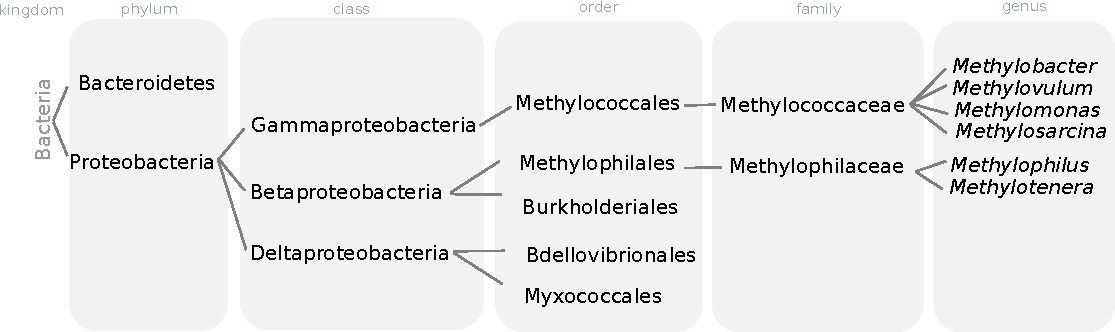
\includegraphics[width=1.0\textwidth]{./tex/chapter2/figures/170311_taxonomy_overview.pdf}
     \begin{singlespace}
     \caption[Taxonomy of microbes known to factor into methane oxidation in Lake Washington sediment.]{
        Taxonomy of microbes that often appear in methane incubations of Lake Washington sediment.
        The family Methylococcaceae is methanotrophic.
        The family Methylococcaceae includes non-methanotrophic methylotrophs.
        Burkholderiales grow on multi-carbon compounds, but in addition, some are methylotrophs.}
     \label{fig:taxonomy}
     \end{singlespace}
\end{figure}

Previous metagenomics and metatranscriptomics studies of Lake Washington sediment have highlighted dominance of the methanotrophic family Methylococcaceae \cite{beck2013LW, beck2014LW, oshkin2015LW, hernandez2015LW}.
These methanotrophs provide substrates for non-methanotrophic methylotrophs to grow \cite{beck2013LW}.
The particular methanotroph species and methylotroph species that dominate the sample is known to be influenced by oxygen availability \cite{hernandez2015LW}.
In previous studies, it was noted that low \ce{O2} tensions select for Methylotenera/Methylobacter partnerships whereas high \ce{O2} tensions select for Methylophilus/Methylosarcina partnerships \cite{hernandez2015LW}.
There is also a revolving cast of non-methylotrops including Burkholderiales and Bacteroidetes \cite{kalyuzhnaya2008Burkholderiales, beck2014LW}.
Better understanding of the metabolic roles that each of these species play, and why certain partnerships tend to form would provide insight into this greenhouse-gas mitigating microbial community.

\subsubsection{Goals of this study}
This study aims to identify the major methanotrophic, methylotrophic, and other microbial species that together enable methane consumption in Lake Washington, and deduce each taxa's contribution to the community metabolism.
Identification of which methanotrophs dominate in natural communities provides insights into how good past isolate studies reflect the true drivers of methane oxidation.
Identification of which metabolic pathways are expressed by these methanotrophs and the accompanying non-methanotrophs informs the mechanism of methane oxidation in this natural system.
Understanding each microbes contribution to the community metabolism allows hypotheses about genetic factors in methanotroph/methylotroph partnerships.

%For example, this study also aims to address the relative importance of two functionally redundant methanol dehydrogenase enzymes: Xox-MDH and Mxa-MDH. (cite).
%TODO: write more about this if I get results in the area.
%TODO: Some methylotrophs only have Xox.  So they are using it, or absent.

% --- How this dataset is poised to address these questions:    Experimental design: (don't make it too methodsy!)
The experimental design chosen to answer these questions is show in in Figure \ref{fig:experimental_design}.

\begin{figure}[H]
\centering
     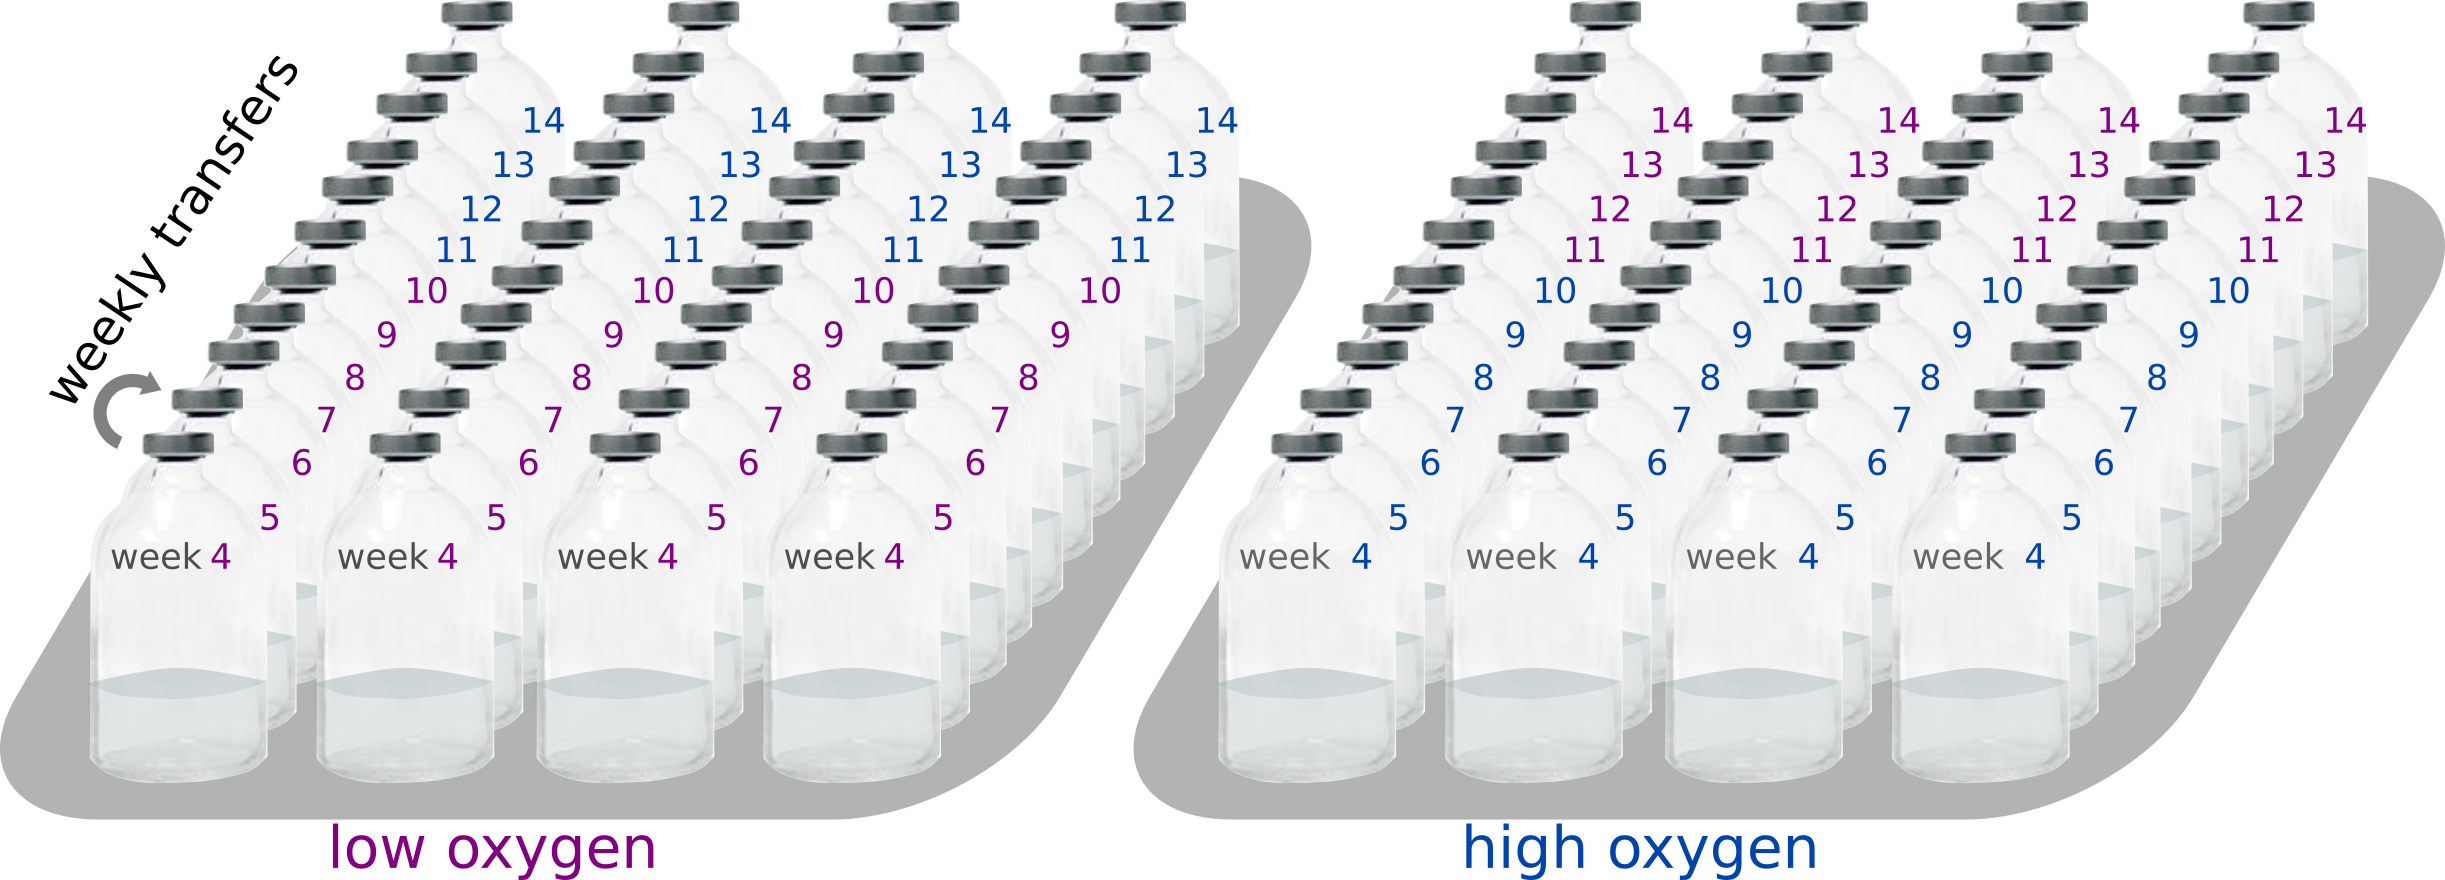
\includegraphics[width=1.0\textwidth]{./tex/chapter2/figures/170311_experimental_design_meta4--2_colors.png}
     \begin{singlespace}
     \caption[Experimental design.]{
        Sediment from Lake Washington, which had been thawed from -80$^o$C and cultured in 8 different bottles,
			half of which were treated with low oxygen, and half of which were at high oxygen (see methods).
		Bottles were serially transferred for a total of 14 weeks.
		The last four bottles in each series are at the opposite oxygen condition of the original experimental design (indicated by bottle number color switch).
		Metagenomes and metatranscriptomes were obtained for weeks 4-14, resulting in 88 metagenomes and 88 metatranscriptomes.
		}
     \label{fig:experimental_design}
     \end{singlespace}
\end{figure}

This relatively simple experimental design, including high degree of replication for studies of this type, was chosen to provide statistical power despite differences across replicates and measurement noise.
Variation across replicates can arise from stochasticity as communities rarefy, and are compounded by the noise-generating steps of nucleic acid extraction, ribosomal RNA removal (in the case of metatranscriptomics), library prep, and the sequencing process.
The most important environmental variable identified so far, the oxygen availability, was modulated while holding all other variables constant.
Availability of sequenced isolate strains from the very ecosystem enhance exploration of the dataset by providing some ground-truth biological facts.
Lake Washington isolates can also be integrated into positive controls for many of the computational methods.

% --- Data sets like this are rare and special.
Though sequencing has become routine in most biological domains, this dataset is exceptional for several reasons.
Having 4 replicates for each experimental condition is much greater than typical metagenomic studies.
Furthermore, most metagenomics/metatranscriptomics studies are single timepoint snapshots, rather than time-series.
Having 11 samples in each series leads to a total of 88 samples.
For each of the 88 samples, untargeted metagenomes and metatranscriptomes were gathered.
These pairs allow exploration of the community without the restriction of referencing cultured strains' genomes.
RNA was depleted, so the majority of our sequencing information is about expressed genes.
In all the dataset totals to 9TB, with approximately XX reads per sample.

\begin{table}[H]
\centering
\begin{tabular}{l | cc}
 %\toprule
        & average \# reads per sample & total \# reads \\
\midrule
	metagenomes & XX & XX \\
	metatranscriptomes & XX & XX \\
%\bottomrule
\end{tabular}
\caption{Total number of un-filtered reads.}
\label{table:sample_read_sizes}
\end{table}

% --- Insights into what's challenging
Despite the size and replication of this dataset, answering the questions outlined above proved challenging.
There are many additional challenges in moving from pure-culture 'omics to meta-'omics, and these challenges were amplified by the large size of the data.
First, the study aims to answer who is there, without the luxury of using reference DNA to align sequencing data to.
Thus, the first task is to assemble reference DNA from the vast number of short sequences provided.
This DNA then becomes the basis for answering both "who is there", and "what are they doing".
Ideally, the assembly yields a small number of long sequences.
More often than not, however, under-sampling of DNA or lack of punctuation in well-sampled (highly abundant) strains leads to fragmented reference DNA.
This fractured reference DNA carries uncertainty and information loss through the rest of the analysis, so care must be taken to interpret all downstream results (discussed in Figure XX).

% -- Tool selection & evaluation is challenging.
Furthermore, tool selection and evaluation is challenging.
As discussed in the introduction, metagenomics and metatranscriptomics of natural microbial communities is a rapidly developing field laiden with methodological challenges.
For each step of inference, there are numerous tools utilizing different approaches one must choose from.
Given that tools perform so differently on different data sets, several tools are usually tried for each step.
For each tool, there are numerous tuning knobs the author encourages exploring, leading to a combinatiorial explosion of potential outcomes for each inference step.
Review papers cannot keep up with the rapid rate of progress; the popular set of tools turns over quicker than every 5 years.
Benchmark studies comparing tools are rare and may be optimizing a different objective than the study at hand.
Tool evaluation is not standardized.

% --- Lack of standards in field
The field also lacks standards for assessing the efficacy of each inference step.
This is in part due to differences in goals across metagenomics/metatranscriptomics studies: some aim for high confidence inference about a specific sub-population such as a novel taxa, whereas others aim to describe the sample more broadly.
Many tools provide only limited insight into their efficacy on your particular dataset.
Care must be taken by the investigators to select the right tools, connect them properly, and evaluate results critically.
Often the trade-offs between tools are not evident until they are tested, and the data is explored with a critical eye.
Success in this field requires iteration as these insights are developed.

% --- So Big!
Furthermore, the size of this dataset is both a blessing and a curse
Yes, the high degree of replication and number of samples per series is essential for identifying hypotheses in messy data.
However, many computational tools are not designed to scale to input data of our size, and fail when used on larger datasets than they were developed for.
While some fail quickly and with clear messages, other simply fail by running indefinitely without the tool either completing its task or aborting.
For some goals, the data can be broken into subsets, processed separately, and re-joined upon completion.
However, not every tool can operate on portions of the data, and extra care is required when stitching together results such that the next tool downstream is blind to such manipulations.
Despite the challenges, this thesis lays out preliminary results addressing both what microbes are present, and what they contribute metabolically.


\section{Metagenomics and Metatranscriptomics}




